%---------------------------------------------------------------------------
% System Decomposition.
%
%---------------------------------------------------------------------------


\section{Decomposition}
\label{sec:ch5_decomposition}

During design stage several high level components have been introduced. All those components, with relationships
between them can be found on Figure~\ref{fig:arch_overall}. Rough description of each component, its role and can be
found in following subsection. Further, more detailed analysis of each component is given in next sections of this
chapter.

What should also be noticed is fact that Figure~~\ref{fig:arch_overall} contains only highest level components. Each
component there should be interpreted as application module, with API shared between provider (component realizing
interface) and consumer (module using given other component) being separate, module, package of actual interfaces.




\begin{figure}[h]
  \centering
  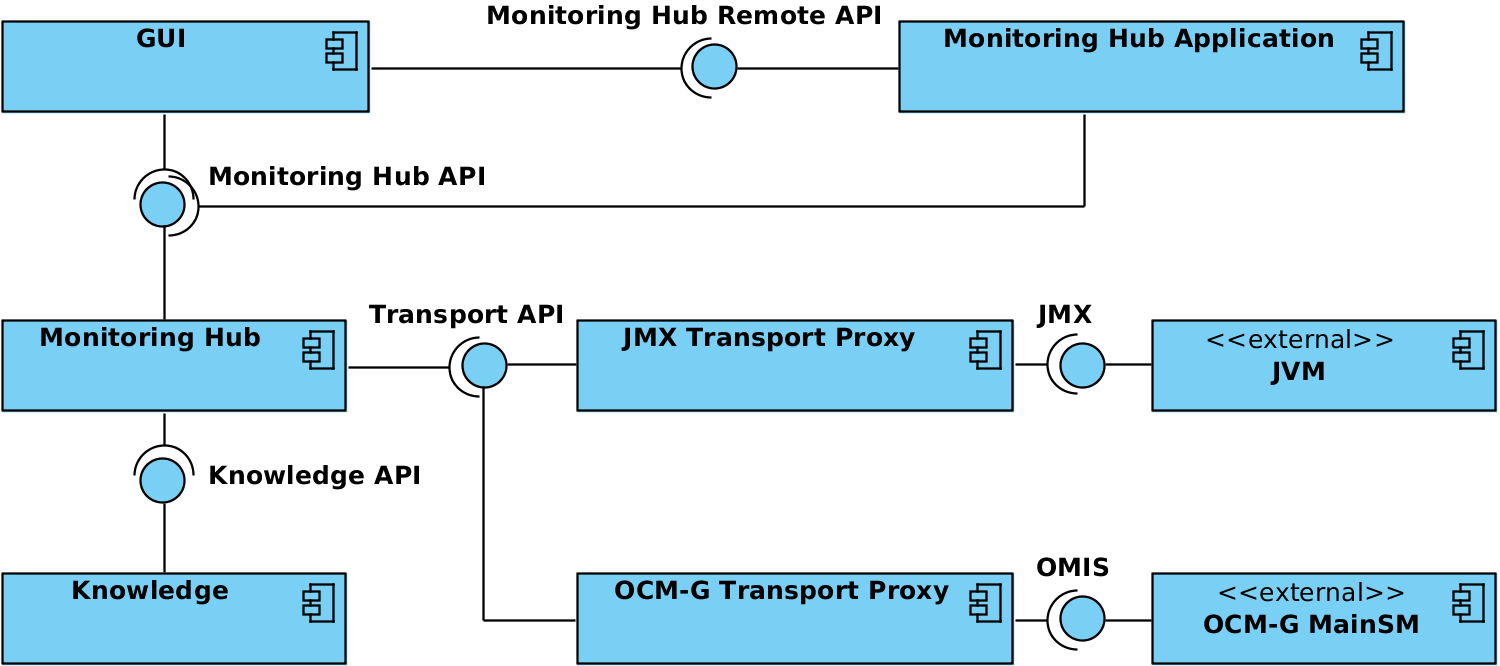
\includegraphics[width=1\textwidth]{arch_overall}
  \caption{Overall system decomposition}
  \label{fig:arch_overall}
\end{figure}

\subsection{Components overview}

Application has been decomposed into following high-level components:

\begin{itemize}
 \item {\bf GUI}~~~~~~~~~~~~~~~~~~~~~~~~~~~~~~~~~~~~~~~~~~~~~~~~~~~~~~~~\linebreak
Graphic User Interface. GUI is standalone, desktop application, used by user directly. Provides to him facilities
allowing management of whole system. Doesn't perform any measurements or analysis, it only gives control over other
components (direct or indirect) and visualizes results of measurements.

GUI application contains embedded Monitoring Hub, which allows system to operate also in smallest scale - single
measuring process with one or more measured processes attached to it directly. Additionally it connects to
Monitoring Hub Application which allows using Monitoring Hub remotely.

 \item {\bf Monitoring Hub}~~~~~~~~~~~~~~~~~~~~~~~~~~~~~~~~~~~~~~~~~~~~~~~~~~~~~~~~\linebreak
Most important component. Contains all logic needed for resources and measurements management. To fulfill it's
duties it uses Knowledge components with one or more transport proxies. At this stage of development only JMX and
OCM-G transport proxies are provided, but current architecture allows ease addition of new proxies. 

Monitoring Hub doesn't work as standalone application. Instead, it is in form of library (Java jar) that is used by
other components that work as processes. Monitoring Hub component is used by GUI (in embedded mode) and by
Monitoring Hub Application.

 \item {\bf Monitoring Hub Application}~~~~~~~~~~~~~~~~~~~~~~~~~~~~~~~~~~~~~~~~~~~~~~~~~~~~~~~~\linebreak
Standalone, command line application (or daemon if possible) that exposes services of Monitoring Hub to other
components, allowing remote access through the network. It can accept remote connections from GUI components.

It's main responsibility is to allow distributed approach to work with system, when using it in medium to large scale.
Having process that is separate, and independent from GUI application, which continuously measures work of long
lasting jobs is crucial to allow measuring system to scale up. 

 \item {\bf Knowledge}~~~~~~~~~~~~~~~~~~~~~~~~~~~~~~~~~~~~~~~~~~~~~~~~~~~~~~~~\linebreak
Knowledge component is responsible for semantic approach. It provides ontology functionalities to Monitoring Hub. It's
responsible for initializing ontology database and response to all queries issued by Monitoring Hub regarding
relationships between resource types, resources or capabilities.

This component is in form of a library that is dependency for Monitoring Hub, and must be included both GUI and
Monitoring Hub Application distributions.


 \item {\bf JMX Transport Proxy}~~~~~~~~~~~~~~~~~~~~~~~~~~~~~~~~~~~~~~~~~~~~~~~~~~~~~~~~\linebreak
Transport proxy component, that is capable to connect to measured JVM process through JMX protocol. It also responsible
for maintenance of mapping between resource types and Java specific entities and capabilities measure requests to
queries that JMX can answer.

 \item {\bf OCM-G Transport Proxy}~~~~~~~~~~~~~~~~~~~~~~~~~~~~~~~~~~~~~~~~~~~~~~~~~~~~~~~~\linebreak
Transport proxy component that connects to OCM-G MainSM monitor, allowing integration with applications monitored
using this system. It's responsibility is similar to the one of JMX Transport Proxy - connect to MainSM, translate
queries given as ontology terms to OMIS specific requests.

\end{itemize}


\subsection{Interfaces overview}

Components to communicate with each and other use following interfaces:

\begin{itemize}
 \item {\bf Monitoring Hub API}~~~~~~~~~~~~~~~~~~~~~~~~~~~~~~~~~~~~~~~~~~~~~~~~~~~~~~~~\linebreak
Interface realized by Monitoring Hub component and used by GUI. Provides facility allowing implementation of all
functionalities related to resources management, as well as measurements. It allows also registration of listeners on
capability values.

 \item {\bf Monitoring Hub Remote API}~~~~~~~~~~~~~~~~~~~~~~~~~~~~~~~~~~~~~~~~~~~~~~~~~~~~~~~~\linebreak
It's derivative of Monitoring Hub API - wraps same set of functionalities, but additionally allows remote access to
them.

 \item {\bf Transport API}~~~~~~~~~~~~~~~~~~~~~~~~~~~~~~~~~~~~~~~~~~~~~~~~~~~~~~~~\linebreak
Common interface realized by all Transport Proxies currently provided, and the one that should be realized to provide
services of additional measuring system.

 \item {\bf Knowledge API}~~~~~~~~~~~~~~~~~~~~~~~~~~~~~~~~~~~~~~~~~~~~~~~~~~~~~~~~\linebreak
Exposes functionalities related to ontology maintenance and usage. Realized by Knowledge component, used by Monitoring
Hub. 
\end{itemize}

\subsection{Most important data flows}



\begin{figure}[h]
  \centering
  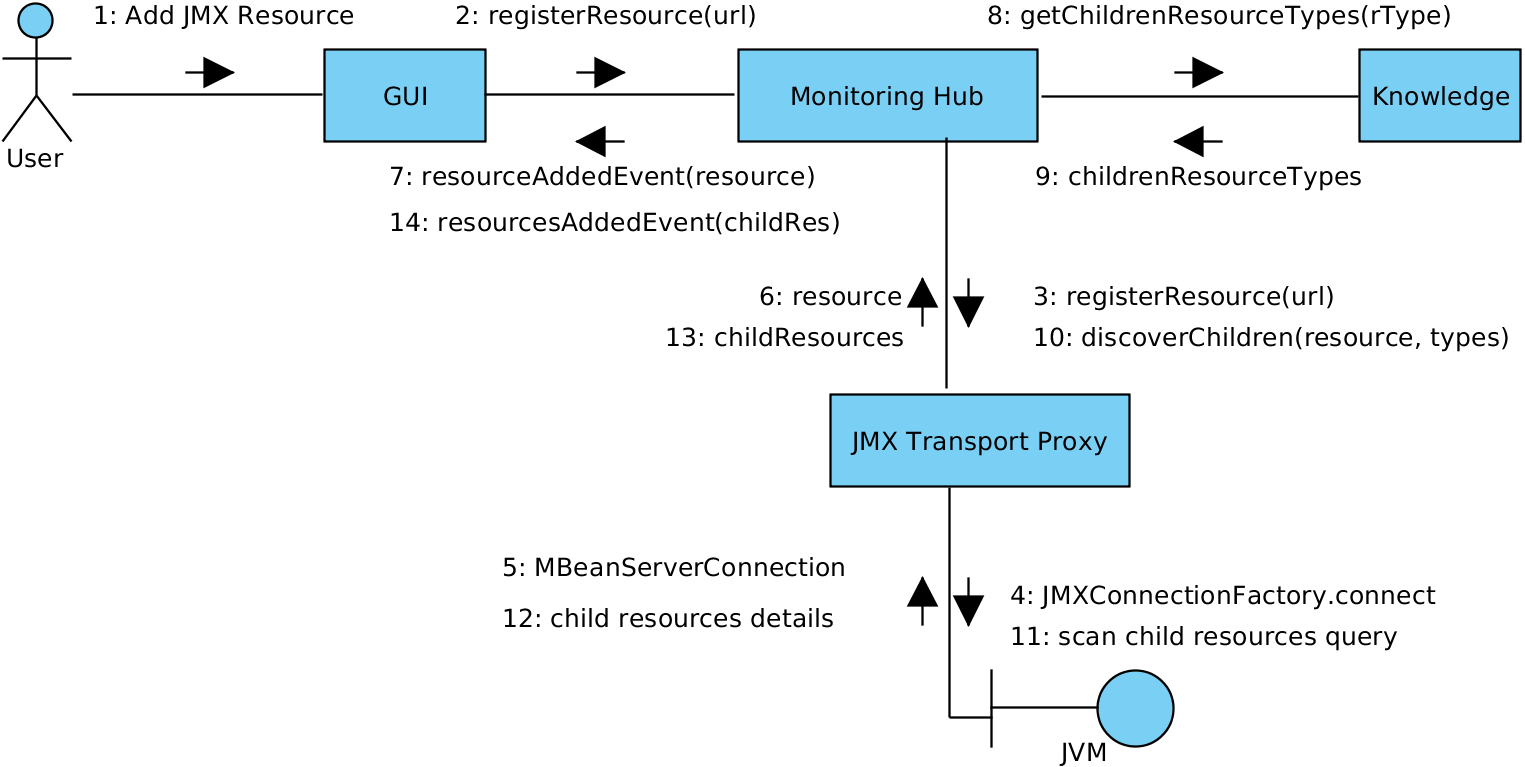
\includegraphics[width=0.9\textwidth]{comm_add_resource}
  \caption{Communication diagram - adding of new resource}
  \label{fig:comm_add_resource}
\end{figure}

Figure~\ref{fig:comm_add_resource} contains communication diagram of messages sequence, exchanged between components to
add new resource. As can be seen, here user is initiator of operation - he performs actions (button click/wizard, not
covered here) needed to add new resource. In next step, GUI sends to Monitoring Hub request to register new resource
with parameters provided by user. Hub then passes request to valid transport proxy. In
Figure~\ref{fig:comm_add_resource} it passes it directly to Jmx Transport Proxy, but that's just an sample. In reality,
it iterates over all registered transport proxies to find the one that supports given resource. In this case, JMX
Transport Proxy tries to initialize connection to JVM using URL provided by user in first step. After successful
connection fully initialized resource is being returned to Monitoring Hub. Knowing that transport proxy has been
properly attached to newly registered resource, Monitoring Hub notifies about new resource all listeners - in this
case GUI component. After issuing this notification, it will try to discover all children of this resource. To
achieve that, it firs calls Knowledge component to get URLs of resource types that can be children of given resource.
With those resource types, Monitoring Hub will request transport proxy to discover children of given resource. 
Again, in this case JMX transport proxy will translate discovery request into JMX queries, to discover child resources.
Discovered children are then returned to Monitoring Hub as resource objects. All those object are registered by Hub and
notification is being sent to listeners - GUI again.


\begin{figure}[h]
  \centering
  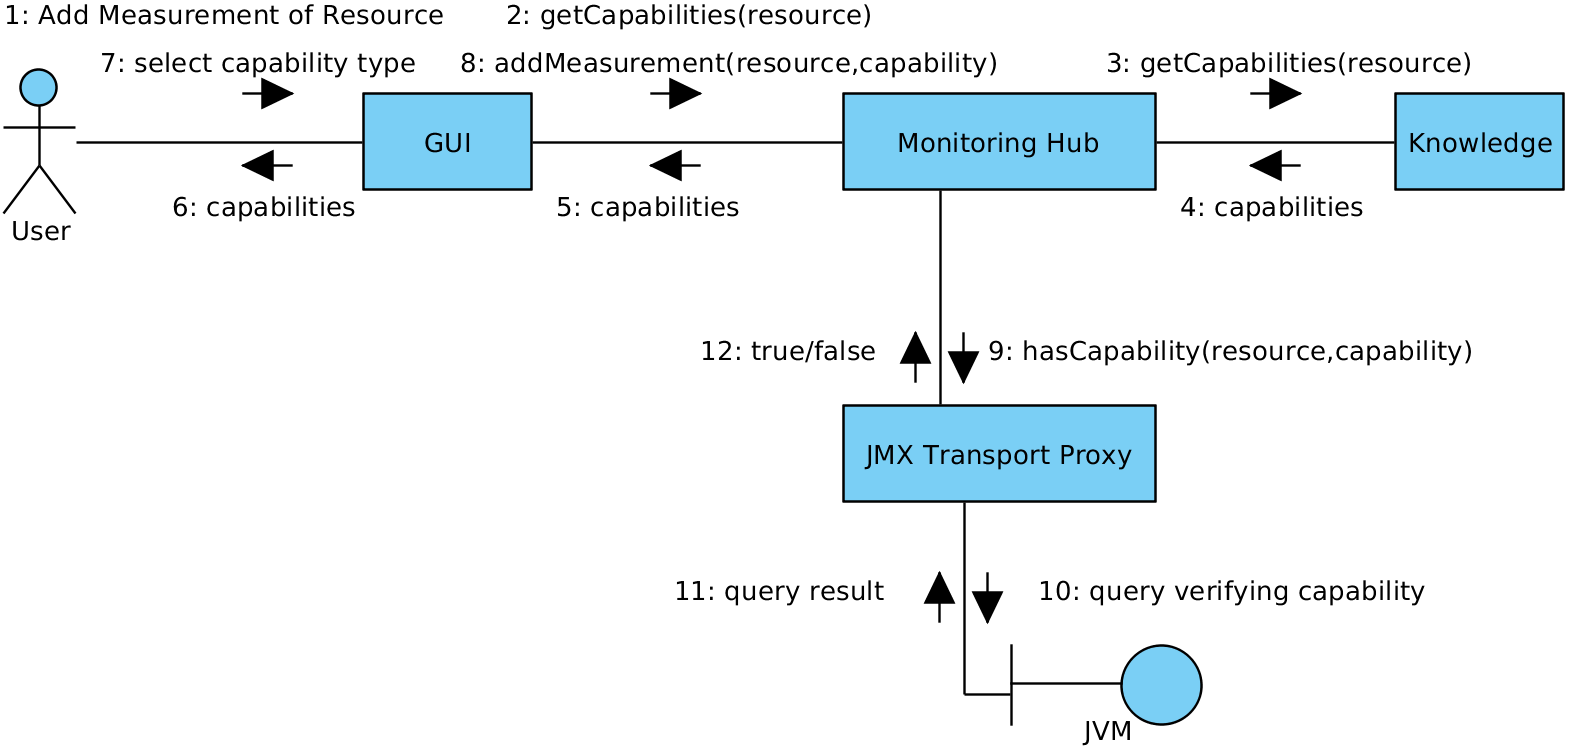
\includegraphics[width=0.9\textwidth]{comm_add_measurement}
  \caption{Communication diagram - adding of new measurement}
  \label{fig:comm_add_measurement}
\end{figure}

Addition of new measurement is a bit more straightforward than adding new resource. All messages exchange needed to
achieve it can be found in Figure~\ref{fig:comm_add_measurement}. Here again, user is initiator of operation. He or she
chooses resource to add measurement of, and clicks appropriate button. With this request processed by GUI, it calls
Monitoring Hub to get all possible capabilities that given resource can have. Monitoring Hub passes this request to
Knowledge component. Then, results goes back GUI, which can render appropriate component, that allows user to select
which capability should be measured. After selecting capability by user, GUI issues request to add new measurement to
Monitoring Hub. It then verifies whether selected capability can be measured with selected resource. It's needed,
because in certain situations it might be impossible. To check this, Monitoring Hub sends verification request to
transport proxy (JMX Transport Proxy in example from Figure~\ref{fig:comm_add_measurement}). After successful
verification, Monitoring Hub initializes scheduler that will poll for capability values - measurement is successful
added.


\begin{figure}[h]
  \centering
  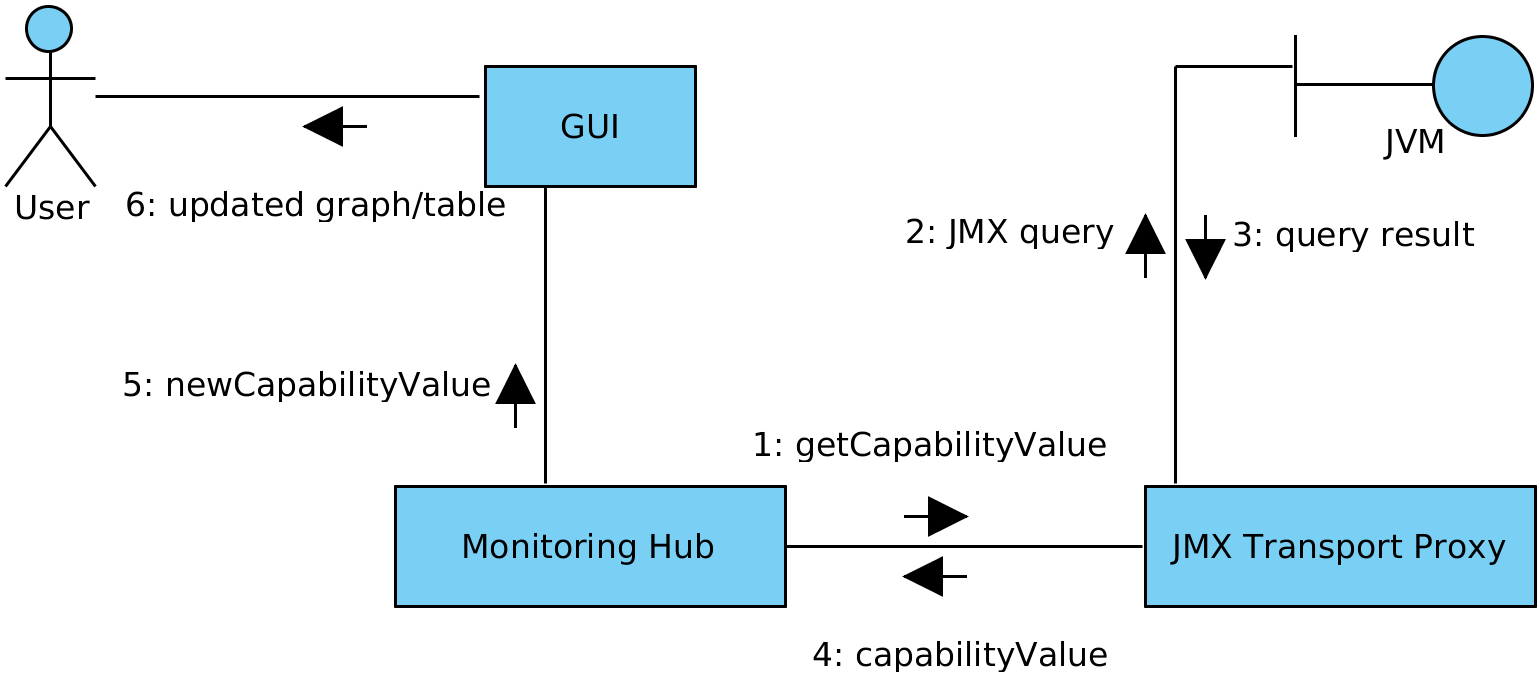
\includegraphics[width=0.7\textwidth]{comm_new_cap_value}
  \caption{Communication diagram - new capability value}
  \label{fig:comm_new_cap_value}
\end{figure}

Publishing new capability values is definitely most frequently used data flow in whole application.
Figure~\ref{fig:comm_new_cap_value} contains it's whole illustration. As can be seen, Monitoring Hub is initiator of
this operation. That's because it manages scheduled jobs responsible for polling of new capability values, and then
pushing to listeners - previously registered GUI components. In first step, Monitoring Hub calls appropriate transport
proxy, which is JMX Transport Proxy in this case, but it's just an example. JMX Transport Proxy maps generic
getCapabilityValue request into specific JMX query, sends the query to monitored JVM and returns result to Hub.
Monitoring Hub uses this result to issue notification dispatched through all registered listeners. GUI, as such a
registered listener, receives event and updates visualization graph, which is being observed by user.


\subsection{Communication protocol}

Communication protocol between components must allow both types of interactions: local, when all components are part
of same process and use same memory space and remote, when one or more components works as a separate process to
others which enforce usage of some kind of network stack to be employed for messages exchange. To make it possible, all
communications will be performed using predefined, plain interfaces, aren't aware communication type. Such a approach
additionally decouples communication from networking protocol being used.

As a general rule for all communications between components, Transfer Object (also known as Value Object) design
pattern will be employed\cite{0131422464}. This allows decoupling content of message from serialization mechanisms
used. Below one may found more details regarding transfer objects used in system. 

% Add vertical spacing
\renewcommand*\arraystretch{1.2}


\begin{table}[h] % ======================== CapabilityValue =====================================
\begin{tabular}{| m{1,5cm} | m{2,5cm} | m{8,5cm} |}
   \hline 
   \cellcolor[gray]{0.9} Field Type & \cellcolor[gray]{0.9} Field Name & \cellcolor[gray]{0.9} Details \\
   \hline 
   Number & numberValue & Numeric value of capability (optional) \\
   Number[] & arrayValue & Vector value of capability (optional)  \\
   ValueType & valueType & Type of capability value - either numeric or vector\\
   Date & gatherTimestamp & Timestamp in UTF, when capability value have been gathered \\
   String & metricsId & Id of measurement to which this capability value belongs \\
   \hline 
\end{tabular}
 \caption{List of members of CapabilityValue Transfer Object}
 \label{tab:TO_CapValue}
\end{table} % ======================== CapabilityValue =====================================

Table~\ref{tab:TO_CapValue} contains list of members of CapabilityValue transfer object. This
object is used to notify listeners (GUI) about new capability value, and acts mostly as container for value, with
additional metadata. Most significant additional property that each CapabilityValue has is gatherTimestamp. With this
property, system can use CapabilityValues, without carrying about implication of processing time on measurements
presentation.

Members of MeasurementDefinition message format can be found in Table~\ref{tab:TO_MeasurementDef}. This object is used
by GUI component to define measurement that should be created during createMeasurement request.



\begin{table}[h] % ======================== MeasurementDefinition =====================================
\begin{tabular}{| m{1,5cm} | m{2,5cm} | m{8,5cm} |}
   \hline 
   \cellcolor[gray]{0.9} Field Type & \cellcolor[gray]{0.9} Field Name & \cellcolor[gray]{0.9} Details \\
   \hline 
   String  & resourceUri &  Uri of resource that is covered by this measurement \\
   String & capabilityUri & Uri of capability that is covered by this measurement \\
   long & updateInterval & Interval in milliseconds defining how frequently value of measurement will be polled \\
   String & id & Identifier of this measurement \\ 
   \hline 
\end{tabular}
 \caption{List of members of MeasurementDefinition Transfer Object}
 \label{tab:TO_MeasurementDef}
\end{table} % ======================== MeasurementDefinition =====================================

Following tables:~\ref{tab:TO_Resource} and \ref{tab:TO_ResourceEvent} contains transfer objects needed by resources
management. Resource transfer object contains complete description of resource managed by system, additionally
MonitoringHub uses ResourceEvent to notify all listeners (GUI mostly) about resource's life cycle events.  

\begin{table}[h] % ======================== Resource =====================================
\begin{tabular}{| m{1,5cm} | m{2,5cm} | m{8,5cm} | }
   \hline 
   \cellcolor[gray]{0.9} Field Type & \cellcolor[gray]{0.9} Field Name & \cellcolor[gray]{0.9} Details \\
   \hline
   String & typeUri & URI of resource's type according to currently used ontology \\
   String & uri & URI of resource in current resources tree hierarchy \\
   Map & properties & Static properties of resource (e.g. OS version) \\
   \hline 
\end{tabular}
 \caption{List of members of Resource Transfer Object}
 \label{tab:TO_Resource}
\end{table} % ======================== Resource =====================================



\begin{table}[h] % ======================== ResourceEvent =====================================
\begin{tabular}{| m{1,5cm} | m{2,5cm} | m{8,5cm} | }
   \hline 
   \cellcolor[gray]{0.9} Field Type & \cellcolor[gray]{0.9} Field Name & \cellcolor[gray]{0.9} Details \\
   \hline
   Type & eventType & Enumeration that defines whether resources in this event have been added  or removed  \\
   List & resources & Collections of resources covered by this event \\
   \hline 
\end{tabular}
 \caption{List of members of ResourceEvent Transfer Object}
 \label{tab:TO_ResourceEvent}
\end{table} % ======================== ResourceEvent =====================================


% Remove vertical spacing
\renewcommand*\arraystretch{1}
